\documentclass[a4paper,12pt]{report}

\usepackage[italian]{babel}
\usepackage{hyperref}
\usepackage{float}
\usepackage{xcolor}
\usepackage{amsmath}
\usepackage{graphicx}

\title{\textbf{Fisica}\\Appunti universitari}
\author{Luca Casadei}
\date{\today}

\begin{document}
	\maketitle
	\tableofcontents
	\chapter{Cinematica}
	Questo capitolo parla del moto dei corpi.\\
	\textbf{Punto}: Se consideriamo un punto, ci interessano le sue coordinate ${X,Y,Z}$ nello spazia, ciascuna coordinata è una funzione nel tempo:
	${X(t),Y(t),Z(t)}$ per ogni istante t il punto si troverà in una certa posizione. Questo è rappresentabile anche attraverso un vettore, che ha anch'esso 3 dimensioni.\\
	\textbf{Misura}: Le coordinate rappresentano una distanza da un'origine nello spazio.
	Nel sistema di riferimento viene rappresentata una curva in forma parametrica.
	\section{Moto rettilineo}
	Nel moto rettilineo ho una retta che ha un verso (orientata) e il punto si muove su questa retta, determiniamo con ${x(t)}$ la posizione del punto sulla retta, definito da una sola coordinata spaziale. Questa funzione è detta \textbf{legge oraria}.
	\begin{figure}[H]
		\centering
		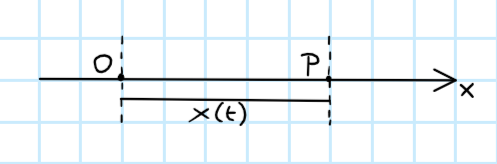
\includegraphics{./immagini/cinematica/figcine1.png}
		\caption{Rappresentazione del moto rettilineo}
	\end{figure}
	\subsection{Velocità}
	Se il corpo si sta spostando per come lo osservo, prendendo due istanti diversi ${t_1,t_2}$ il corpo è in posizioni diverse ${x_1,x_2}$, possiamo definire la velocità media come: ${v_m = \frac{\Delta_x}{\Delta_t} = \frac{x_2 - x_1}{t_2 - t_1}}$.\\
	Questa si basa su dei ${\Delta}$ macroscopici, se ${t_2}$ si avvicina a ${t_1}$, il ${\Delta}$ diventa sempre minore e il limite rappresenta effettivamente la derivata.\\
	Inoltre essa è la pendenza della retta secante a quella che rappresenta il movimento, se riduco $t_2$ fino ad arrivare a $t_1$ ottengo la \textbf{velocità istantanea}.\\
	Vediamo quindi come arrivare a questa velocità: se consideriamo il coefficiente angolare $m_{sec} = {{\frac{f(x_0 + h) - f(x_0)}{x_0 + h - x_0}} \Rightarrow {\frac{(x_0 + h) - f(x_0)}{h}}}$ come si può notare questo è il rapporto incrementale che dobbiamo utilizzare per ottenere questa volta la velocità istantanea (quindi in un istante), che è rappresentata dal coefficiente angolare della retta tangente al punto dell'istante di nostro interesse, procediamo quindi con: $m_{tg} = {\lim\limits_{h\to0}(\frac{f(x_0 + h) - f(x_0)}{h})} = {\frac{df}{dx}(x_0)} = {\lim\limits_{\Delta t\to0}(\frac{\Delta x}{\Delta t})} = v_{\text{ist}}$ come si può vedere ho ottenuto la derivata, con la quale posso calcolare la velocità in un certo istante.
	\subsubsection{Classificazione delle velocità in base al grafico della funzione}
	\begin{itemize}
		\item \textbf{Nessun moto}: Se la funzione è costante, la retta è parallela all'asse delle ascisse e non abbiamo quindi alcun movimento.
		\begin{figure}[H]
			\centering
			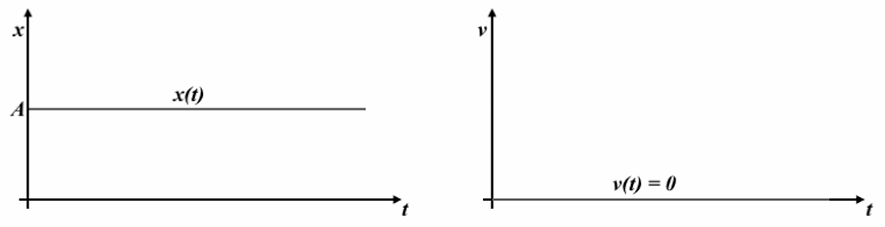
\includegraphics[width=300pt]{./immagini/cinematica/figcine2.png}
		\end{figure}
		\item \textbf{Velocità costante}: Se il diagramma orario è una retta e non presenta curve, la sua derivata (velocità) è semplicemente la retta tangente di tutti i suoi punti, la cui pendenza è 0. In questo caso:\\
		$x(t) = A + Bt$;\;\;\;$v(t) = B = \frac{\Delta x}{\Delta t}$
		\begin{figure}[H]
			\centering
			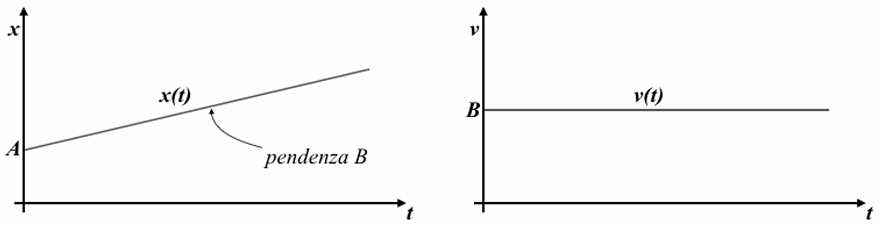
\includegraphics[width=300pt]{./immagini/cinematica/figcine3.png}
		\end{figure}
		\item \textbf{Velocità non costante}: Nel caso in cui la velocità cambia nel tempo (ad esempio se cresce sempre all'aumentare del tempo), allora si avrà una curva e non una retta nel diagramma orario.
		\begin{figure}[H]
			\centering
			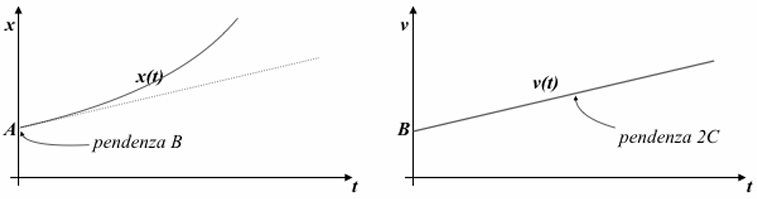
\includegraphics[width=300pt]{./immagini/cinematica/figcine4.png}
		\end{figure}
	\end{itemize}
	Possiamo notare che matematicamente per arrivare alla velocità considerando le 3 coordinate di un punto è che: ${{X = A + B(t) + C(t^2)} \Rightarrow {v = B + C(t)}}$.
	\subsubsection{Ricavare la legge oraria dalla velocità}
	Ovviamente si può ricavare $x(t)$ facendo l'integrale di $v(t)$, che è il contrario della derivata, con qualche accorgimento. Devo infatti prestare particolarmente attenzione al fatto che l'integrale da fare è quello definito, quindi descritto da un intervallo.\\\\
	Possiamo effettuare la seguente trasformazione:\\\\
	${\frac{dx}{dt} = v(t)}\Rightarrow\\{{dx} = {v(t)dt}} \Rightarrow\\{\int_{x_0}^{x}(dx')} = {\int_{t_0}^{t}(v(t')dt')} \Rightarrow\\{x-x_0} = {\int_{t_0}^{t}(v(t')dt')}\Rightarrow\\{x} = {x_0} + {\int_{t_0}^{t}(v_0(dt'))}\Rightarrow\\x(t) = x_0 + v(t-t_0)\Rightarrow \mathcolor{red}{x(t) = x_0 + vt}$\\\\
	Quando abbiamo un movimento di un corpo e dobbiamo sapere la sua posizione a seguito di una certa velocità, dobbiamo sapere da dov'è partito, quindi un'istante di tempo che ci dica dove sia all'inizio, per questo nella formula compare $x_0$, dato che l'integrale è definito questo è il punto come consideriamo come quello di partenza, che tipicamente prendiamo come $0$. Passare invece dalla legge oraria alla velocità non richiede nessun parametro aggiuntivo.\\ \textit{Attenzione}: Se la funzione della velocità è discontinua (ad esempio quando si torna indietro), la funzione non è derivabile, quindi si devono considerare due leggi del moto differenti, prima dell'urto e dopo l'urto.
	\subsection{Accelerazione}\label{ss:accelerazione}
	Possiamo distinguere accelerazione media e accelerazione istantanea come nella velocità.\\\\
	$a_{m} = \frac{\Delta v}{\Delta t}$\\
	$a = \frac{dv}{dt} = \frac{d^2x}{dt^2}$\\
	$a = 0 \Longleftrightarrow v$ è costante.\\
	$dv = a(t)dt \Longrightarrow \Delta v = \int_{v_0}^{v}dv = \int_{t_0}^{t}a(t)dt$\\
	$v(t) = v_0 + \int_{t_0}^{t}(a(t))dt$\\\\
	Se $a$ è costante ho un \textbf{moto rettilineo uniforme} definibile con: $x(t) = x_{0} + \int_{t_{0}}^{t}(v(t'))dt = X_0 \int_{t_0}^{t}[v_0 + a(t-t_0)]dt = x_0 + \int_{t_0}^{t}v_0dt + \int_{t_0}^{t}a(t - t_0)dt \Longrightarrow \mathcolor{red}{x(t) = x_0 + v_0(t - t_0) + \frac{1}{2}a(t - t_0)^2}$\\\\
	Se però non abbiamo informazioni sul tempo, e vogliamo considerare la velocità in funzione della distanza invece che il tempo ($v(x)$ invece che $v(t)$), elaboro le informazioni nel seguente modo:\\
	$a = \frac{dv}{dt} = {\frac{dv}{dx}\frac{dx}{dt}} = v(\frac{dv}{dx}) \Rightarrow\\adx = vdv$ passo poi all'integrale $\int_{x_0}^{x}(a)dx' = \int_{v_0}^{v}(v)dv = \int_{x_0}^{x}(a(x))dx' = \frac{1}{2}v^2 - \frac{1}{2}v^2_{0} \Longrightarrow\\\mathcolor{red}{v^2 = v^2_0 + 2a(x -x_0)}$
	\subsubsection{Unità di misura}
	$[L] \longrightarrow m \rightarrow Km$\\
	$[T] \longrightarrow s \rightarrow h$ (hours), $d$ (days), $y$ (years)\\
	$[v] = [LT^{-1}] \longrightarrow \frac{m}{s} \rightarrow \frac{Km}{h}$\\
	$[a] = [LT^{-2}] \longrightarrow \frac{m}{s^2}$
	\subsection{Caduta di corpi gravi}
	Consideriamo uno spazio bidimensionale (la caduta è considerata completamente in verticale).\\
	Dobbiamo considerare in questo caso l'accelerazione di gravità sulla terra, definita generalmente come: $g = 9,81\frac{m}{s^2}$, questo è un moto uniformemente accelerato caratteristica di qualsiasi gravo sulla terra se verso il basso, verso l'alto sarà la sua controparte negativa $-g$. Si possono presentare diversi casi:
	\begin{itemize}
		\item Un corpo cade da un'altezza h con $v_0 = 0$\;\;\;$x_0 = h$\;\;\;$t_0 = 0$\\Valgono quindi le seguenti funzioni a partire da quelle precedentemente ottenute (vedi \ref{ss:accelerazione}).
		\begin{equation}
			\begin{cases}
				v(t) = -gt	\\
				x(t) = h - \frac{1}{2}gt^2
			\end{cases}
		\end{equation}
		Queste sono espresse in funzione del tempo, ma come abbiamo fatto in precedenza, possiamo ricavarle anche in funzione dello spazio:
		\begin{equation}
			\begin{cases}
				v(x) = \sqrt{2g(h-x)}	\\
				t(x) = \sqrt{\frac{2(h-x)}{g}}
			\end{cases}
		\end{equation}
		Se vogliamo ottenere il tempo o la velocità partendo dallo spazio, considerando $x = 0$ possiamo ottenere dalle ultime due formule:
		\begin{itemize}
			\item Tempo di caduta: $t_c = \sqrt{\frac{2h}{g}}$
			\item Velocità al suolo: $v_c = \sqrt{2gh}$
		\end{itemize}
		\item Un corpo cade da altezza $h$ con $v_0 < 0$ (verso il basso): Qui abbiamo le condizioni iniziali $x_0 = h;$\;\;\;$v_0 = -v_i$ se $(v_i > 0);$\;\;\;$t_0 = 0$, sono quindi valide le seguenti espressioni:
		\begin{equation}
			\text{In funzione del tempo:}
			\begin{cases}
				v(t) = -v_1 - gt\\
				x(t) = h - v_1t - \frac{1}{2}gt^2
			\end{cases}
		\end{equation}
		\begin{equation}
			\textit{In funzione dello spazio:}
			\begin{cases}
				v(x) = \sqrt{v_1^2 + 2g(h-x)}\\
				t(x) = -\frac{v_1}{g} + \sqrt{\frac{v_1^2}{g^2} + \frac{2(h-x)}{g}}
			\end{cases}
		\end{equation}
		Anche in questo caso ricaviamo il tempo e la velocità di arrivo al suolo.
		\begin{itemize}
			\item Tempo di caduta: $t_c = -\frac{v_1}{g} + \sqrt{\frac{v_1^2}{g^2} + \frac{2h}{g}}\rightarrow$ in questo caso abbiamo scartato la soluzione negativa, perché il tempo non può essere negativo.
			\item Velocità al suolo: $v_c = \sqrt{v_1^2 + 2gh}$
		\end{itemize}
		\item Un corpo viene lanciato verso l'alto $(v_0 > 0)$, partendo dal suolo. In questo caso le condizioni iniziali sono: $x_0 = 0;$\;\;\;$v_0 = v_2 > 0;$\;\;\;$t_0 = 0;$
		\begin{equation}
			\text{In funzione del tempo:}
			\begin{cases}
				v(t) = v_2 - gt\\
				x(t) = v_2t - \frac{1}{2}gt^2
			\end{cases}
		\end{equation}
		\begin{equation}
			\text{In funzione dello spazio:}
			\begin{cases}
				v(x) = \pm\sqrt{v_2^2 - 2g(x)}\\
				t(x) = \frac{v_2}{g}\pm\sqrt{\frac{v_2^2}{g^2} - \frac{2x}{g}}
			\end{cases}
		\end{equation}
		Si presenta in questo caso un più o meno, deriva dal fatto che il corpo passa due volte nella stessa posizione, una volta mentre sta salendo e la seconda volta mentre sta scendendo.
		\begin{itemize}
			\item Tempo di caduta: $t_c = \frac{v_2}{g}\pm\frac{v_2}{g}$
			\item Velocità al suolo: $v_c = \pm v_2$
		\end{itemize}
		La rappresentazione grafica di quest'ultimo tipo di moto è data dall'interpretazione che inizialmente il corpo si trova al livello del suolo con $t = 0;$\;\;\;$v = v_2$ e successivamente $t = \frac{2v_2}{g}$ con $v = -v_2$.
		\begin{figure}[H]
			\centering
			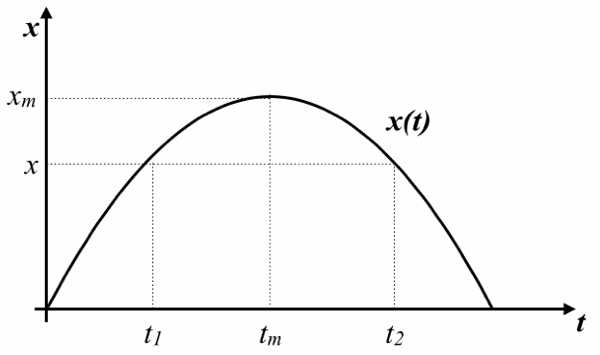
\includegraphics[width=200pt]{./immagini/cinematica/figcine5.png}
		\end{figure}
	\end{itemize}
	
	\section{Moto nello spazio}
	Quando non abbiamo un moto rettilineo (in una dimensione) possiamo descrivere il moto in maniera più generale nello spazio attraverso le dimensioni spaziali. La posizione di un elemento nello spazio è individuata da un vettore posizione:
	\begin{figure}[H]
		\centering
		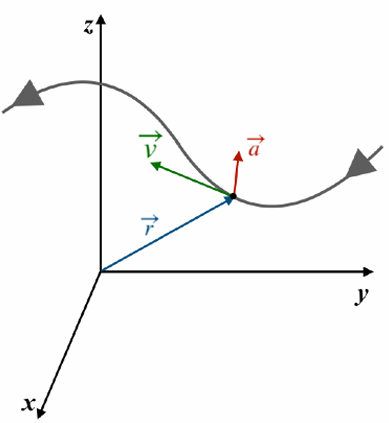
\includegraphics[width=200pt]{./immagini/cinematica/figcine6.png}
		\caption{$\vec{r}(t) = x(t)\hat{i} + y(t)\hat{i} + z(t)\hat{k}$}
	\end{figure}
	\begin{itemize}
		\item \textbf{Velocità}: I concetti di velocità media e velocità istantanea sono analoghi a quelli di una dimensione:\\
		dati $\vec{r_1} = \vec{r_1}(t)$ e $\vec{r_2} = \vec{r_2}(t_2)$ definisco lo spostamento $\Delta\vec{r} = \vec{r_2} - \vec{r_1}$ che avviene in un certo intervallo temporale $\Delta t = t_2 - t_1$, quindi (ricordando che $v_m$ è la velocità media e $v$ quella istantanea):\\
		$\vec{v_m} = \frac{\Delta \vec{r}}{\Delta t}$;\;\;\;\;
		$\vec{v} = \lim\limits_{\Delta t \to 0}(\frac{\Delta\vec{r}}{\Delta t}) = \frac{d\vec{r}}{dt}$\\
		Se vogliamo rappresentare le componenti cartesiane:\\$\vec{v} = v_x\hat{i} + v_y\hat{j} + v_z\hat{k} = \frac{d(x\hat{i} + y\hat{j} + z\hat{k})}{dt}$ e scomponendo quest'ultima frazione possiamo ottenere: $v_x = \frac{dx}{dt};$\;\;\;$v_y = \frac{dy}{dt};$\;\;\;$v_z = \frac{dz}{dt}$
		\item \textbf{Accelerazione}: Procediamo in modo analogo con l'accelerazione:\\
		$\vec{a_m} = \frac{\Delta\vec{v}}{\Delta t};$\;\;\;\;$\vec{a} = \lim\limits_{\Delta t\to0}(\frac{\Delta\vec{v}}{\Delta t}) = \frac{d\vec{v}}{dt}$\\
		$a_x = \frac{dv_x}{dt};$\;\;\;\;$a_y = \frac{dv_y}{dt};$\;\;\;\;$a_z = \frac{dv_z}{dt}$\\
		$a_x = \frac{d^2x}{dt^2};$\;\;\;\;$a_y = \frac{d^2y}{dt^2};$\;\;\;\;$a_z = \frac{d^2z}{dt^2}$\\
		È possibile produrre un'accelerazione che varia soltanto la direzione della velocità $\vec{v}$ e non il modulo $|\vec{v}|$.
	\end{itemize}
	\chapter{Dinamica}
	Perché un corpo si muove in un determinato modo?
	\appendix
	\chapter{Esercizi}
	\section{Cinematica}
	\subsection{In slide di teoria}
	\begin{itemize}
		\item \textit{Guido l’automobile a $43 Km/h$ per $5.2 Km$ su una strada rettilinea. Resto senza benzina e 
			percorro a piedi $1.2 Km$ in $27$ minuti, fino al distributore. Qual è stata la mia velocità media? 
			Disegnare anche un grafico di $x(t)$.}\\\\
			$v(x) = 43 \frac{Km}{h}$\\
			Spazio percorso è: $x = x_1 + x_2 = (5,2 + 1,2)Km = 6,4Km$\\
			$v_m = \frac{\Delta x}{\Delta t} = \frac{x- x_0}{t - t_0} = \frac{6400}{t}\frac{m}{s}$ Ci manca da trovare $t = t_1 + t_2$\\
			$t_1 = (\frac{1}{43} * 5,2)\frac{h}{Km} * Km = 0,1209h = 435,24s$\\
			$t_2 = 27m = 27 + 60 = 1620s$\\
			Concludendo: $v_m = \frac{6400}{2055,24}\frac{m}{s} = 3,1139\frac{m}{s}$\\
			Posso ricavare la legge oraria facendo l'integrale definito della velocità, ottenendo $x(t) = vt$
	\end{itemize}
	
\end{document} 